%!TEX root = *.tex
%%%%%%%%%%%%%%%%%%
% カウンタのリセット
\setcounter{figure}{0}
% 問題文
図1のように,
傾きの角$30^\circ$のなめらかな斜面上に質量$m$の台車が置かれ,
その台車には軽く伸び縮みしない糸の一端が取り付けられている.
その糸のもうー端は,
斜面の上端に固定された定滑車と,
床と軽いばねでつながれた動滑車を介して,
天井に取り付けられている.
なお,台車,定滑車,動滑車,糸は,すべて同一の鉛直面内にあり,
台車から定滑車までの糸は斜面と平行,
定滑車から動滑車および動滑車から天井までの糸は鉛直で,
糸がたるむことはないものとする.
また,2つの滑車は軽く,なめらかに回るものとする.



台車が静止しているときの位置をつり合いの位置とする.
図1のように,このつり合いの位置から,
斜面の最下点までの距離を$L$とする.
なお,距離$L$,ならびに,台車から定滑車までの距離は,
後述する単振動による台車の振幅に対して,
十分に長いものとする.
また,ばね定数を$k$,重力加速度の大きさを$g$とする.
空気抵抗や摩擦は無視できるものとして,
以下の問いに答えなさい.
ただし,解答に用いる物理量を表す記号は,
問題文中に与えられているもののみとする.


\begin{figure}[H]
  \centering
  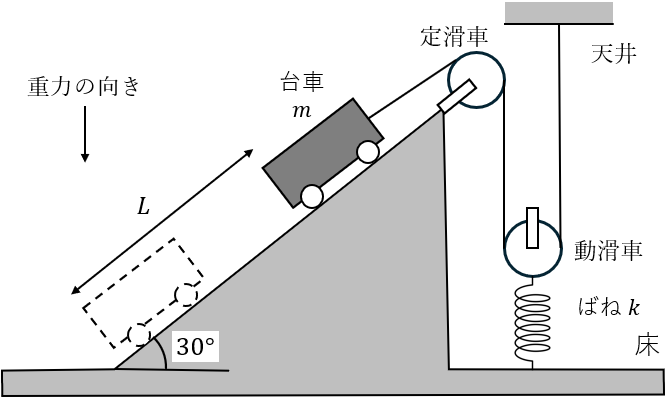
\includegraphics[width=.6\columnwidth]{../graphs/chiba_23_1.png}
  \caption{}
\end{figure}

\begin{enumerate}[(1)]
  \setlength{\leftskip}{-1zw}
  \setlength{\itemindent}{1zw}\setlength{\labelsep}{0.5zw}
  \setlength{\labelwidth}{1zw}\setlength{\leftmargin}{1zw}
  \setlength{\itemsep}{0.5\baselineskip}
  \item つり合いの位置において台車が静止しているときの,糸が天井を引く力の大きさを求めなさい.
  \item つり合いの位置において台車が静止しているときの,ばねの自然長からの伸びを求めなさい.
  \item 台車がつり合いの位置にあるときの,ばねの弾性力による位置エネルギーを求めなさい.
\end{enumerate}



台車の下端を手で支えながら斜面に沿って図1の右上方向にゆっくり移動させ,
ばねが自然長になったところで静かに台車から手をはなしたところ,
台車は斜面に沿って単振動した.



\begin{enumerate}[(1)]
  \setlength{\leftskip}{-1zw}
  \setlength{\itemindent}{1zw}\setlength{\labelsep}{0.5zw}
  \setlength{\labelwidth}{1zw}\setlength{\leftmargin}{1zw}
  \setlength{\itemsep}{0.5\baselineskip}
  \addtocounter{enumi}{3}
  \item 単振動をしている動滑車と台車の振幅をそれぞれ求めなさい.
  \item 単振動をしているときの台車の最大の速さを求めなさい.
  \item この単振動の周期を求めなさい.
\end{enumerate}



ばねが自然長になり台車から手をはなした時刻を$t=0$とする.
手をはなした後,ある時刻で台車に取り付けられた糸を切断する.
なお,糸を切断する直前と直後で,台車の運動エネルギーや位置エネルギーは変化しないものとする.
次の2つの問いについてそれぞれ答えなさい.



\begin{enumerate}[(1)]
  \setlength{\leftskip}{-1zw}
  \setlength{\itemindent}{1zw}\setlength{\labelsep}{0.5zw}
  \setlength{\labelwidth}{1zw}\setlength{\leftmargin}{1zw}
  \setlength{\itemsep}{0.5\baselineskip}
  \addtocounter{enumi}{6}
  \item 手をはなした後,台車がつり合いの位置を2回通過した直後に糸を切断した場合を考える.
  台車は,糸の切断後も,斜面に沿って運動を続けた.
  糸を切断した後に,台車の速さが最初に0になるまでのつり合いの位置からの斜面方向の移動距離と,速さが最初に0になったときの時刻を求めなさい.
  \item 糸の切断時刻を変えることで,台車が斜面の最下点に到達するときの速さを最大にしたい.そのための切断時刻と,台車が斜面の最下点に到達するときの速さを求めなさい.なお,切断時刻は,$t>0$の最も早い時刻とする.
\end{enumerate}







% メモ
\begin{comment}

\end{comment}


%%%%%%%%%%%%%%%%%%
